%% chapter 3

\chapter{单细胞RNA测序数据处理流程}

\section{将原始测序数据转化为基因表达矩阵}
  在将生物样品进行测序后,我们会得到内含测序数据的fastq文件。但fastq文件是由高通量测序产生的输出文件,我们不能直接使用它进行数据挖掘。在这项研究中我们使用CellRanger将其转化为基因表达矩阵,并基于此开展下游分析。

  CellRanger是一组分析管道,用于处理Chromium单细胞数据以对齐读取、生成Feature-Barcode矩阵、执行聚类和其他辅助分析等。CellRanger有四个处理管线与3'单细胞基因表达解决方案及其相关产品有关,我们在这里只关注常用的cellranger mkfastq与cellranger count,其对应流程如图\ref{fig:cellranger-workflow}所示。cellranger mkfastq的主要作用是将Illumina测序生成的原始碱基检出(BCL)文件转化为fastq文件。cellranger count对cellranger mkfastq获取的fastq文件执行对齐、过滤、Barcode计数以及UMI计数,我们使用其产生的计数矩阵进行下游分析。

\begin{figure}[!htb]
  \centering
  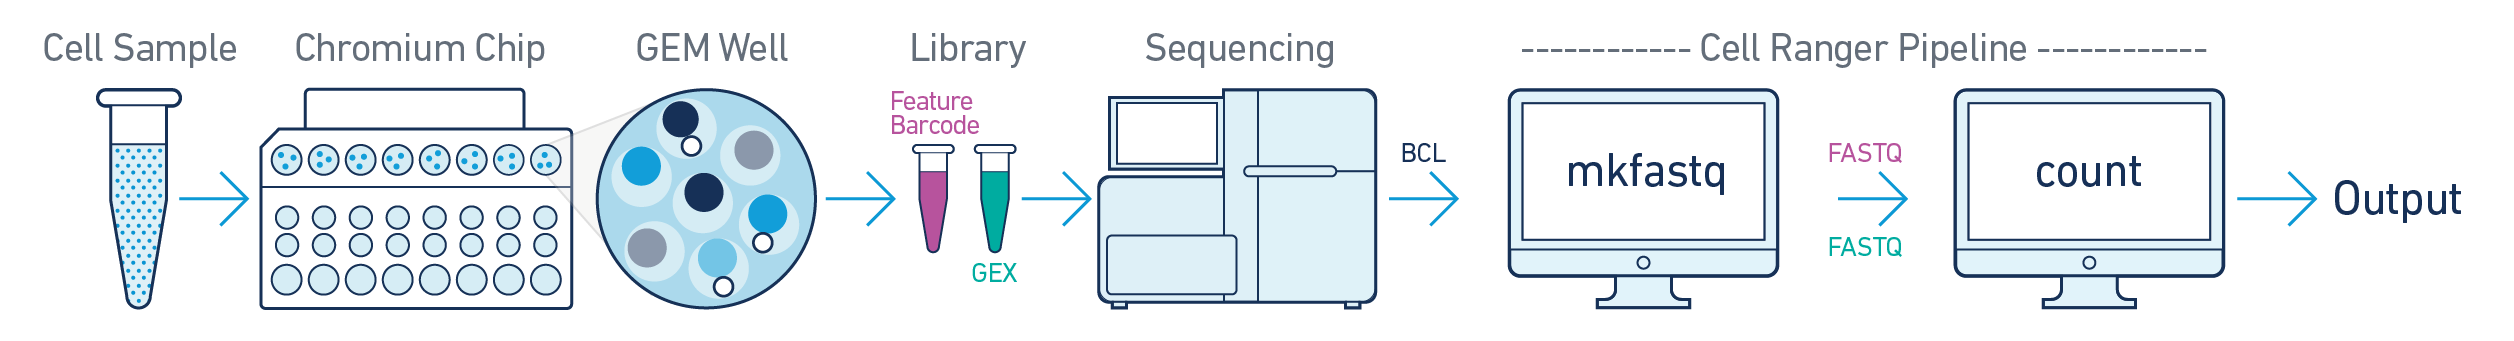
\includegraphics[width=0.8\textwidth]{figs/cellranger-workflow.png}
  \caption{CellRanger工作流程}
  \label{fig:cellranger-workflow}
\end{figure}

\section{对基因表达矩阵进行质量控制}
  对基因表达矩阵进行质控的主要目的是去除制备生物样品和单细胞RNA测序过程中引入的噪音。例如,在进行单细胞RNA测序的过程中,受限于测序芯片的技术条件,会有一定比例将两个细胞吹到同一个测序单位中,又或是使细胞破损等。为了保证下游分析结果的正确性,我们必须将这些离群点检测出来并将其去除。

  目前进行质量控制的主流方法还是阈值法,即对基因表达矩阵在细胞水平(Cell-level QC)、基因水平(Feature-level QC)以及变量水平(Variable-level QC)依据所处理生物数据特性人为设置生物合理的阈值。正常情况下,所检测到的线粒体RNA占所检测到RNA总量的5\%以下,如果高于这个值便可能是在测序的过程中出现细胞破损,导致细胞质RNA外流。但是这种情况也不是绝对的,比如在肌肉细胞中代谢旺盛,所检测到的线粒体RNA占比便会高于此值,因此我们需要针对组织的特异性设定不同的阈值。

  在质量控制之后,我们还可以去除一些已知功能且与研究不相关的RNA(比如核糖体RNA、线粒体RNA),以避免其对下游分析的影响。

\section{依据基因表达矩阵进行聚类}
  在对基因表达矩阵进行质量控制之后,为探求单细胞层级的异质性,我们可以依照其基因表达的差异将其聚类为不同的簇,并鉴定不同簇上的基因marker,为之后的分析提供基础的生物见解。Seurat v3\cite{butler2018integrating,stuart2019comprehensive}建议的初步处理流程是:归一化、特征选择、放缩、线性降维、构建最短近邻图、Leiden聚类和UMAP可视化。
\subsection{特征选取}
  特征选取是在Feature-Barcode矩阵(或者说Gene-Cell矩阵)中计算每个基因的方差,并对其进行排序,选取其中具有较高方差的基因集合(即,它们在某些细胞中高表达,而在其他细胞中低表达)用于下游线性降维。这里使用一些方差较大基因的原因在于,从信息学的角度来看,方差越大的变量蕴含的信息越多。同时,Brennecke等人在2013年的一项研究\cite{brennecke2013accounting}表明在下游分析中关注这些基因有助于去除技术噪声,以在单细胞数据集中突出显示生物信息。线性降维也是基于此原理,对数据进行进一步的筛选,去除方差较低成分的噪声影响。
\subsection{Leiden聚类算法}
  Leiden聚类\cite{traag2019louvain}是整个初步处理流程的关键一步,其依据线性降维结果构建的最短近邻图挖掘其中的群落结构,其原型是Louvain聚类算法\cite{blondel2008fast}。我们下面会详细介绍Louvain算法的局限以及Leiden算法的改进。

  Louvain算法和Leiden算法都是基于图数据的群落发现算法,其灵感源于modularity的优化。其中,modularity是一个定义在$[-1/2,1]$的比例值,用于度量群落内部边缘相对于群落外部边缘的相对密度。对于加权图,modularity由公式(\ref{equ:graph-modularity})定义:
\begin{equation}
  \label{equ:graph-modularity}
  Q = \frac{1}{2m}\sum_{ij}\left[A_{ij} - \frac{k_{i}k_{j}}{2m}\right]\delta(c_{i},c_{j})
\end{equation}
其中,$A_{ij}$表示节点$i$和$j$之间边的权重,$k_{i}$和$k_{j}$分别是连接到节点$i$和$j$的边的权重之和,$m$是图中所有边缘权重的总和,$c_{i}$和$c_{j}$是节点的群落,$\delta$是Kronecker函数(如果$x=y$,$\delta(x,y)=1$,否则为0)。从理论上优化此值会导致给定网络节点的最佳分组,但这在计算上并不可行。因此使用启发式算法,通过迭代来近似modularity的最大值,Louvain算法和Leiden算法都是属于这种形式。

   在Traag等人2019年的一项工作\cite{traag2019louvain}中,实验证据表明Louvain算法得到的分区中会存在连接不良的群落,甚至内部断开的群落。而且他们证明在使用Louvain算法时,该问题在实践中经常发生。在Louvain算法中存在这样一种情况:一个节点在其旧群落中充当不同部分连接的桥梁,但是却可能在群落更新过程中被移动到另一个群落,从其旧群落中删除这样的节点会断开旧群落的连接。Louvain算法可能假设旧群落的其他节点也会移动到该新群落,但事实并非如此,尽管旧群落已经断开连接,但其他节点仍可以与其群落保持牢固的联系,如图\ref{fig:louvain-prob}所示。

\begin{figure}[!htb]
  \centering
  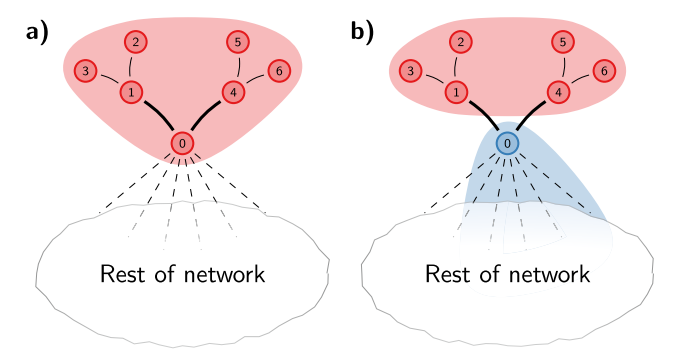
\includegraphics[width=0.8\textwidth]{figs/louvain-prob.png}
  \caption{Louvain算法存在的问题}
  \label{fig:louvain-prob}
\end{figure}

  Leiden算法的改进主要在于利用了加快节点局部移动\cite{ozaki2016simple,bae2017scalable}以及将节点移动到随机邻居\cite{traag2015faster}的思想。Leiden算法由三个阶段组成:(1)节点的局部移动;(2)分区的细化;(3)基于细化的分区进行网络聚合。

  在算法的第一阶段,首先将网络中每个节点分配给其自己对应的群落。然后,对每个节点$i$,计算将其从自身的群落移除并将其移至每个邻居节点$j$对应群落所带来的modularity变化。这两步的公式比较相似,其中将节点$i$移至其邻居节点$j$对应群落所带来modularity的变化由公式(\ref{equ:modularity-change})定义:
\begin{equation}
  \label{equ:modularity-change}
  \Delta{Q} = \left[\frac{{\Sigma}_{in} + 2k_{i,in}}{2m} - \left(\frac{{\Sigma}_{tot} + k_{i}}{2m}\right)^{2}\right] - \left[\frac{{\Sigma}_{in}}{2m} - \left(\frac{{\Sigma}_{tot}}{2m}\right)^{2} - \left(\frac{k_{i}}{2m}\right)^{2}\right]
\end{equation}
其中,${\Sigma}_{in}$是节点$i$将要移入群落中所有连接的权重之和,${\Sigma}_{tot}$是节点$i$将要移入群落中所有连接到节点的权重之和,$k_{i}$是节点$i$的加权度,$k_{in}$是节点$i$与其将要移入群落中所有节点的连接权重之和,$m$是网络中所有连接权重之和。利用加快节点局部移动\cite{ozaki2016simple,bae2017scalable}的思想,仅计算与节点$i$相连所有群落中刚修改群落的modularity,其余沿用以前的计算值。

  在算法的第二阶段产生的分区$\mathcal{P}_{refined}$是Louvain算法对应阶段生成分区$\mathcal{P}$的细分。分区$\mathcal{P}$中的群落可以分为分区$\mathcal{P}_{refined}$中的多个群落。在进行合并的过程中,节点$i$并没有像Louvain算法中那样贪婪地与最大化modularity的群落合并,而是随机选择任何可以增加modularity的群落进行合并。modularity的增加越大,选择该群落的可能性就越大\cite{traag2015faster}。选择群落的随机性允许更广泛的探索分区空间。此外,仅当节点$i$与分区$\mathcal{P}$中的群落充分良好地连接时,才将其与分区$\mathcal{P}_{refined}$中的群落合并,从而避免分区存在连接不良的群落。

  在算法的第三阶段,将第二阶段得到的每一个群落折叠为单个节点,并在此基础上建立新的网络。这时,新群落节点上的自环表示同一群落节点之间的所有连接,而群落节点之间的加权边表示同一群落多个节点到不同群落节点的连接。在新网络创建完毕后,其结果可以重新用于算法的第一阶段,进行迭代,最终得到聚类结果。

  总之,Leiden算法可以保证产生的分区中不会存在连接不良的群落。在Leiden算法被迭代使用时,它会收敛到一个分区,在该分区中,可以确保所有群落的所有子集都属于局部最优分配。因此,Leiden算法可以提供准确的聚类见解,供下游分析使用。

